%!TEX root = ../article/Journal_SelfCalibration.tex

\section{Methods}
\label{sec:methods}

\subsection{Experimental Protocol}

The usability of the self-calibration approach was tested under an experimental protocol demonstrated in a prior work \cite{iturrate13}. The protocol consisted of a $5\times5$ squares grid, a virtual cursor, and a goal location (see Fig. \ref{fig:protocol}). The cursor performs five different instantaneous actions: move one position up, down, left, right; and a goal-reached action, represented as concentric circumferences (see Fig. \ref{fig:protocol}b). The time between two actions (inter-action interval) was random within the range $[3, 3.5]$ s. The role of the subjects was to assess the cursor actions as correct when the cursor performed $(i)$ a movement towards the goal position, or $(ii)$ a goal-reached action over the goal position; or as incorrect otherwise (see Fig. \ref{fig:protocol}c). These assessments generated the associated evoked potentials for both correct and error conditions (i.e., error-related potentials, ErrP \cite{chavarriaga2014errare}). Note that the goal position was known by the user, but it was unknown by the device. The users were instructed not to move their eyes during the cursor actions, and to restrain blinks only to the resting periods. The experiment duration was fixed to 500 actions performed by the device, with rest intervals every 10 actions. Every time the device reached a target, the target was changed to a different position, with the sequence of target positions the same for all the subjects. The total length of the experiment was around 50 minutes. For more details about the protocol, please refer to \cite{iturrate13}.

\begin{figure}[!tbp]
\centering
%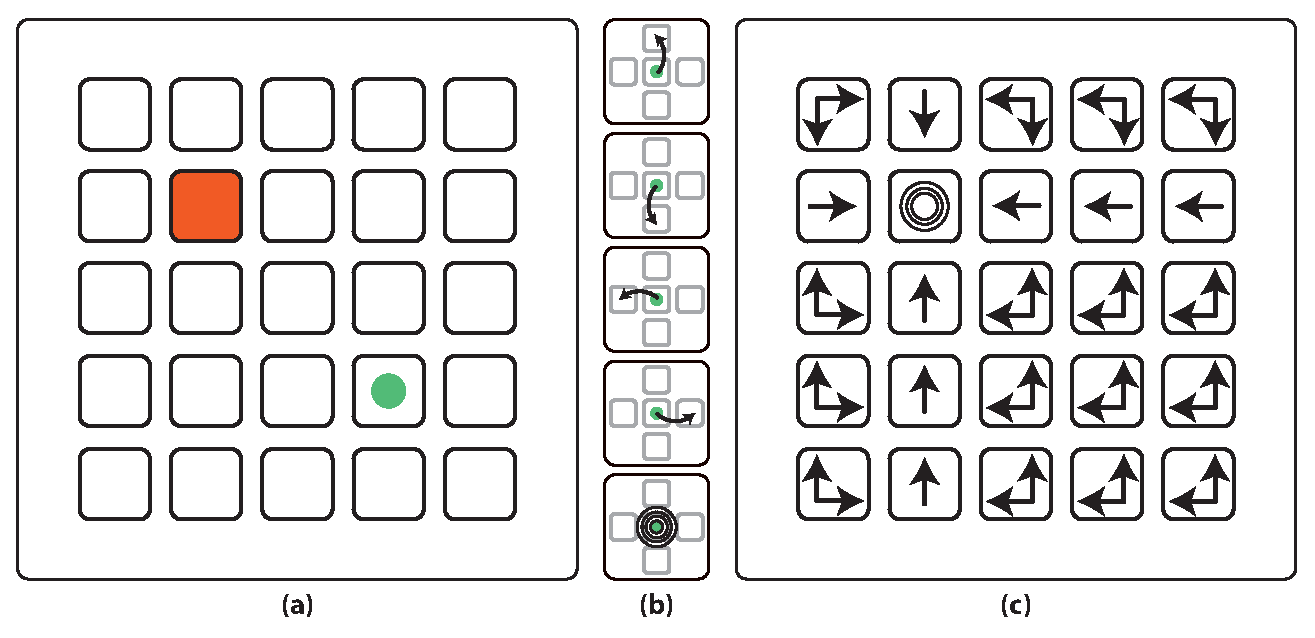
\includegraphics[width=\columnwidth]{figures/experimentalProtocol.eps}
\caption{\label{fig:protocol} \textbf{Experimental protocol} (a) Experimental protocol. The protocol showed a $5\times5$ grid with a virtual cursor (green circle) and a goal location (shadowed in red). (b) The cursor could perform five different actions (from top to bottom, move one position up, down, left, right, or performing a goal-reached action). (c) Correct actions (i.e. optimal policy) from each state for the goal exemplified in (a). Extracted from \cite{iturrate13} with permission.}
\end{figure}


Eight subjects (mean age $28 \pm 1.55$ years) participated in the experiments after the protocol was approved by the Institutional Review Board of the University of Zaragoza. All participants were asked to read and sign an informed consent form to participate in the study. The participants were seated on a comfortable chair one meter away from a computer screen that displayed all the information related to the experiment. 
%
%Subjects were assigned accordingly to three different groups, depending on their experience as BMI users: $(i)$ naive BMI users (3 subjects); $(ii)$ usual BMI users, but with no expertise on the current protocol (2 subjects); and $(iii)$ usual BMI users that participated in the protocol previously (see \cite{}), following an standard calibration (2 subjects).
%
For the executed experiments we used an unsupervised self-calibration approach (c.f. section \ref{sec:zerocalibration}) to simultaneously train the error-related potentials (ErrP) \cite{chavarriaga2014errare} classifier  and solve the task (i.e., reach the target position). The data recorded during the experiments is publicly available, and can be downloaded from \url{https://github.com/flowersteam/self_calibration_BCI_plosOne_2015}.

\subsection{Data recording and feature extraction}

EEG signals were recorded from 16 fronto-central active electrodes using a gTec system, with the ground on AFz and the reference on the left earlobe. EEG data were digitized with a sampling frequency of 256 Hz, power-line notch filtered, and band-pass filtered at $[1, 10]$ Hz. The data acquisition and online processing was developed under a self-made BCI platform. 
%
In this work, ErrP features were extracted from channels Fz, FCz and Cz within a time window of $[200,800]$ ms downsampled by a factor of 8 (being 0 ms the action onset), forming a vector of $57$ features \cite{chavarriaga2010learning}. 

%\todo{After every agent's action, the brain signals from the user are recorded via a computer using a gTec system. To build our feature vector we consider two fronto-central channels (FCz and Cz) in a time window of $[200,700]$ ms (being 0 ms the action onset of the agent) and downsampled the signal to $32$ Hz. Each element of the feature vector is the value in microvolts of the signal at the corresponding time.}


% \cite{chavarriaga2010learning, iturrate13}. In this section 
 
 
\subsection{Supervised decoding of error potentials}

Before describing the self-calibration method for error-based control, we briefly describe here the supervised approach \cite{chavarriaga2010learning, iturrate13} which will be later extended to an unsupervised setting.
%
The decoding of the EEG signals is done using a Gaussian classifier.  The signals are modeled using an independent multivariate normal distribution for each class (i.e. correct denoted as $c$ or error as $w$) \cite{lotte2007review,blankertz2010single}, $\mathcal{N}(\mu_c, \Sigma_c), \mathcal{N}(\mu_w, \Sigma_w)$.  $\theta_k$ denotes  the set of parameters of each class  $\{\mu_k, \Sigma_k\}$ where $k\in\{c,w\}$.
%
The covariance matrices $\Sigma_c$ and $\Sigma_w$ are shrinked  ($\lambda = 0.5$) to avoid overfitting when using a large number of features compared to the training number of samples\cite{ledoit2004honey}. 

The probability of a label given a signal is obtained using the Bayes' rule:
%
\begin{eqnarray}
    p(l = j|e,\theta_j) &=& \frac{p(e|l = j, \theta_j)p(l = j)}{\sum_{k = c,w}{p(e|l = k,\theta_k)p(l = k)}}
  %  &=& \frac{p(e|l=l_j, \theta)}{\sum_{k = c,w} p(e|l=l_k)} \nonumber
\end{eqnarray}
where $e$ represents the features extracted from the brain signal, $j\in\{c,w\}$ is one of the two classes to be decoded.
%
As we do not have a priori knowledge on the user intended assessment of the action, we assume all labels are equi-probables, i.e. $\forall k,~p(l = k) = 0.5$. 
%
In this supervised setting, an estimation of the parameters $\hat{\theta}$ is obtained using a set of pairs of signals and labels prior to the actual use of the brain signals. 

\subsection{Error-potential based control}
\label{sec:errpcontrol}
Once trained, the decoder of the previous section can be used to control a device based on the user's assessment of the behavior of the device \cite{iturrate13}. 
%
The control task is modeled as a Markov decision process (MDP). An MDP is defined by a triplet $(s,a,r)$  where $s\in S$ and $a\in A$ represent the states and actions, and $r$ represents the reward.  Actions modify the state of the system according to the corresponding transition model $p(s'\mid s,a)$. In our grid world protocol, the state represents the cell in the grid and  $p(s'\mid s,a)$ is simply a deterministic transition up, down, left, right, or performing a goal-reached action from the current state $s$ according to the action $a$. The reward function encodes the task, in our case it assigns positive reward to the goal state and zero reward to the others. Given this reward function, it is possible to compute the optimal policy (i.e. a function that gives you the action to execute at each state) that maximizes the accumulated reward. 

Under the assumption that the user follows optimal policies, the ErrP detector can be used to identify the user intended task $\xi = t$ among a finite set of tasks $t = 1,\ldots,T$. Note that this assumption does not contradict the fact that we also assume a non-informative a priori for the labels, as the latter will vary among optimal policies and will depend on the planner.

The rationale of the algorithm is the following: the actions of the device that agree with the optimal policy will not generate error responses, while those that do not follow the policy will. This can be implemented as a recursive filter to identify the task based on the signals $e$ obtained when executing action $a$ in state $s$:
%
\begin{eqnarray}
p(\xi=t|e, s, a, \hat{\theta}) & \propto & p(e |s, a, \hat{\theta}, \xi=t) p(\xi=t)
\label{eq:1}
\end{eqnarray}
%
where  $p(e |s, a, \hat{\theta}, \xi=t)$ needs to take into account the probability of each possible class $k$ given the target $\xi=t$, the current state $s$ and the action $a$ executed by the machine:
%
\begin{eqnarray}
p(e |s, a, \hat{\theta}, \xi=t) =  \sum_{k = c,w} p(e |l = k, \hat{\theta}) p(l = k| s, a, \xi=t)
\label{eq:2}
\end{eqnarray}

The previous estimate simply assigns a higher likelihood to those tasks with whom the brain signals are more coherent. Fig.  \ref{fig:protocol}c shows the optimal policy for a given task, that is, the actions that should not generate error potentials if this is the user's intended task. The posterior distribution is then used to control the device to the most likely goal using a planning algorithm or greedy heuristic (see \cite{iturrate13} for further details).


\subsection{Self-calibration control}
\label{sec:zerocalibration}
%
This section presents a self-calibrated algorithm that eliminates the need of  calibration prior to the control task. This is a self-calibration approach since it estimates $\theta$ in an unsupervised manner during operation.
%
Self-calibration control can be achieved by exploiting the structure of the task space, namely the  labels that the optimal policy of each task assigns to each state-action pair. These learned labels can be used to train a decoder for each possible task. The remaining question is how to select among the different tasks. For this purpose, we define the following pseudo-likelihood function \cite{grizou2014interactive}:
%
\begin{eqnarray}\label{eq:pseudo1}
\lefteqn{P(D_M | \xi=t) \approx \prod_{i=1}^M p(e_i | s_i, a_i, \xi=t, D_{-i})}  \\ \label{eq:pseudo2}
&=& \prod_{i=1}^M \sum_{k=w,c}  p(e_i | l=k, \xi=t, D_{-i})  p(l=k | s_i,a_i, \xi=t).
\label{eq:pseudo}
\end{eqnarray}
%
where $D_M$ represents the history of triplets $\{a_i, s_i, e_i\}$ up to time $M$.
The pseudo-likelihood is built using a leave-one-out cross-validation strategy to evaluate the likelihood $p(e_i | s_i, a_i, \xi=t, D_{-i})$ of each signal $e_i$ based on a model learned with all the other signals and corresponding actions and states denoted by $D_{-i}$. For a given target hypothesis $\xi=t$, the labels associated to the signals in $D_{-i}$ can be estimated (i.e. $p(l=k | s_i,a_i, \xi=t)$), enabling the training of a target-specific classifier for each task $\xi=t$. In a nutshell, Eq. \ref{eq:pseudo} assigns higher likelihood to tasks in which their optimal policies match the labels predicted with the model learned with $D_{-i}$. As detailed in \cite{grizou2014interactive}, the underlying assumption is that the subject is coherent throughout the experiment, providing similar signals for the same set of labels.

The pseudo-likelihood is computed from two terms. $p(l=k|s_i,a_i,\xi=t)$ represents the probability distributions of the labels according to a task, the executed action, and the current state. This term only depends on what action is correct at each state according to task $\xi=t$.   

The other term, $p(e_i | l=k,\xi=t, D_{-i})$, represents the likelihood of the signal given the label provided by the task and the previous history. In principle, one could use directly the same likelihood model as in Eq. \ref{eq:2}, with $\theta$ estimated from $D_{-i}$. However, such a model results in very fast convergence and a high sensitivity to outliers (e.g. incorrect assessments by the user). In order to improve the robustness of the method, we propose to marginalize out $\theta$  using a non-informative (Jeffrey's) prior (see \cite{gelman2003bayesian}, page 88). The resulting likelihood function is a t-student distribution with heavier tails:

\begin{eqnarray}
p(e| l=k,\xi=t, D_{-i}) & = & t_{n-d}\left(e | \mu_k,\frac{\Sigma_k (n+1)}{n(n-d)}\right)
\end{eqnarray}

where $\mu_k$ and $\Sigma_k$ are the corresponding empirical mean and covariance matrix, $n$ is the number of signals, and $d$ is the dimensionality of a signal feature vector.
%
%\todo{Furthermore, $p(l_c | l, \theta_{-i})$ is approximated by the corresponding confusion matrix of the classifier based on $\theta_{-i}$. It is the probability that the classifier itself is reliable in its prediction. \ref{eq:pseudo1}.}

As in the calibrated case, the device can use the task estimates to select the next action greedily according to the corresponding optimal policy \cite{iturrate13}. However, this strategy is prone to fail during the initial stages due to the large uncertainty introduced by the lack of calibration. To alleviate this difficulty, we incorporate this uncertainty in the decision making and use a look-ahead planning based on \cite{grizou2014interactive}.

Unlike the calibrated case, we do not only have uncertainty on the tasks but also on the signal models. Indeed, each task is associated with a different set of signal-label pairs leading to a different classifier. Hence our agent must collect data to discriminate between tasks but also to understand the structure of the signal in the feature space. These two sources of uncertainty can be unified as a measure of uncertainty on the signal space, as described in \cite{grizou2014calibration}, which can be approximated on the label space through a sampling procedure \cite{grizou2014interactive}.

%\todo{Should we put the math that are commented in the tex file in annex?}
% We note $\theta_{\xi_t}$ the classifier associated to task $\xi_t$, i.e. trained on all signals-labels pairs available. We note from Eq.\ref{eq:2}:
% \begin{eqnarray}
% J^{\xi_t}(s,a,e) = p(e |s, a, \theta_{\xi_t}, \xi_t)
% \end{eqnarray}
% And $J^{\xi}(s,a,e)$ the vector $[J^{\xi_1}(s,a,e), \ldots, J^{\xi_T}(s,a,e)]$.

% We compute the uncertainty of one state-action pair given a signal $e$ as the weighted variance of $J$ with weights $W^{\xi} = [W^{\xi_1}, \ldots, W^{\xi_T}]$ being the weight or probability associated to each task (see section~\ref{sec:confidence}):
% \begin{eqnarray}
% U(s,a|e) = weightedVariance(J^{\xi}(s,a,e), W^{\xi})
% \label{eq:planningOneSignal}
% \end{eqnarray}
% with:
% \begin{eqnarray}
% weightedVariance(x,w) = \frac{\sum_{i} w_i (x_i - weightedMean(x,w))}{\sum_{i} w_i}
% \label{eq:weightedVariance}
% \end{eqnarray}
% with:
% \begin{eqnarray}
% weightedMean(x,w) = \frac{\sum_{i} w_i x_i}{\sum_{i} w_i}
% \label{eq:weightedMean}
% \end{eqnarray}

% The uncertainty for a state-action pair is given by:
% \begin{eqnarray}
% U(s,a) & = & \int_{e} U(s,a|e) p(e) de
% \end{eqnarray}
% which we approximate by summing values of $U(s,a|e)$ for different signals $e$:
% \begin{eqnarray}
% U(s,a) & \approx & \sum_{e} U(s,a|e) p(e)
% \label{eq:planning}
% \end{eqnarray}
% with $p(e)$ assumed uniform.

The agent will then target areas of higher uncertainty, to reduce it by collecting more evidence in these areas. To do so, the uncertainty is computed for each state-action pair and used as a reward function to be maximized by the agent (using value iteration \cite{barto1998reinforcement}).
%\begin{eqnarray}
%a_{i+1} = \argmax_a Q_{i}(s,a)
%\end{eqnarray}
%with $Q_i$ is the optimal action-value function at step $i$ computed using Value Iteration and given our uncertainty measure as a reward function.
The system follows the optimal policy for this reward function and switches to a pure exploitation of the task, ignoring the uncertainty, after reaching the desired confidence level (see section~\ref{sec:confidence}).

\subsection{Practicalities}
We now describe some implementation details that were used in the experimental evaluation of the method.  The code is available under a GNU GPL license and can be found at \url{https://github.com/jgrizou/lfui}.

\subsubsection{Power information}
One  critical difficulty of learning from unlabeled signals is for cases where the signals can be interpreted in a symmetric way. In other words, it is possible to obtain the same likelihood by switching the labels. Such misinterpretation is possible in environments with symmetric properties (see \cite{grizou2014interactive} for reaching tasks and \cite{Kindermans2012a,kindermans2014true} for a speller). For the domain of our experiments the symmetries can be disambiguated using the goal reached action, but, in general, symmetric tasks (e.g. opposite corners) will be hard to discriminate and might produce an inconsistent agent behavior.

Prior information about the differences in power between correct and error signals can be used to increase the robustness of the method -- helping to remove world symmetries (e.g. equal likelihood for models with symmetric labels). 
In single trial classification power spectral information results in lower performance than temporal features, but their combination produces more robust detectors \cite{Omedes13ErrPFreq}.
%
However, in our case it is possible to exploit the fact that EEG signals associated to the error class have on average higher power than the ones associated to the correct class.

This information is added to the pseudo-likelihood model of Eq. \ref{eq:pseudo} as follows. The average power information of each class is computed as  the weighted mean of the signals' power. The weights are the probabilities of the label given the signal and the class parameters 
%
\begin{eqnarray}
p_k(\xi=t) = \frac{\sum_{i = 1}^{M} p(l = k | e_i , \theta_k) ~~ e_i^T e_i}{\sum_{i = 1}^{M} p(l = k | e_i , \theta_k)}.
\label{eq:powerCorrect}
\end{eqnarray}
%
with $\theta_k$ the corresponding parameters of each class $k$, and the power computed as the inner product of $e_i$.
%
The pseudo-likelihood is multiplied by the ratio of the power associated to the error class over the power of the correct class:

\begin{eqnarray}
 \bar{P}(D_M | \xi=t) = P(D_M | \xi=t) \frac{p_w(\xi=t)}{p_c(\xi=t)},
\label{eq:power}
\end{eqnarray}

which assigns, given two symmetric labeling, higher probability to the one where the average power of error  signals is larger.  

\subsubsection{Identifying the goal}
\label{sec:confidence}
A practical issue when running this algorithm is to decide when the task has been successfully identified. This decision has to take into account the uncertainty about the task. We use a thresholding method and define as $W^{t}$ the minimum of pairwise normalized likelihood between tasks $\xi=t$ and all other tasks: 
%
\begin{eqnarray}
W^{t} = \min_{x~\in~{1, \ldots, T} \smallsetminus \{t\}} \frac{P(D_M | \theta, \xi=t)}{P(D_M | \theta, \xi=t) + P(D_M | \theta, \xi=x)}
\label{eq:weight}
\end{eqnarray}

When it exists a task $\xi=t$ such that $W^{t}$ exceeds a threshold $\beta \in [0.5,1]$ we consider that it is the one the subject has in mind.

Once a task is identified with confidence, the device switches to a greedy policy following the optimal one to reach the estimated goal. Once there, it starts a new task. At this point the device can use the ErrP signals of the previous task as prior information. Indeed, it assigns to the signals the labels of the optimal policy of the identified task.  Note that this prior information is used by the device for all the subsequent error potentials and it results on faster task identification since the classifier parameters are better estimated from the beginning \cite{grizou2014interactive}. In fact, when tasks are correctly identified, the resulting classifier is equivalent to a calibrated one trained with a similar number of ErrP signals. 

\subsection{Self-calibration control analysis}

Firstly, the recorded potentials during the online experiment were studied to assess whether their characterization was similar to those obtained in previous works. Notice that, contrary to classical calibration approaches where the error ratio remained fixed \cite{chavarriaga2010learning, iturrate13}, the error ratio in our approach could not be fixed due to the exploration algorithm and the unsupervised nature of the problem. For this analysis, signals for each condition (error and correct movements performed by the device) were grand averaged for the time window $[-200, 1000]$ ms, where 0 ms represents the action onset.

Secondly, the self-calibration online task was analyzed with the following metrics: number of steps to reach the first target; total number of (incorrect or correct) targets reached during the whole experiment (500 steps) and number of correct and incorrect targets reached. To evaluate the learning progress during the first target,  the instantaneous error rate was computed as a moving average over the last 10 actions. Finally, we compared the quality of the labels acquired by the self-calibration approach with the one that would be obtained using a supervised calibration method. Note that, when the device reaches an incorrect target, some signals are incorrectly labeled (those corresponding to states whose optimal action differ from the intended target). To this end, we computed the percentage of labels estimated correctly by the self-calibration approach and the ten-fold accuracy obtained using these labels, and compared it to the ten-fold accuracy obtained with ground-truth labels.

Thirdly, the proposed approach was compared with standard calibration procedures. In order to perform this comparison, the important factors to analyze are the quality of the signals acquired, and the labels quality learned from the self-calibration procedure. In principle, if both the signals acquired and labels learned are equivalent to those of a standard calibration, the performance of the system should also be equivalent. To this end, we took advantage of the overlap of three subjects between the current work and our previous work where the protocol was the same but following a classical supervised calibration \cite{iturrate13}. For this analysis, we compared first the quality of the EEG signals in terms of grand averages (error minus correct grand averages); as well as the accuracies obtained during the online control phase following the standard calibration versus the accuracy obtained during the self-calibration session.

Finally, we performed an offline analysis to compare the self-calibration online results with a standard calibration using the same signals acquired during the online experiment. The number of calibration trials required for each subject was estimated by splitting the dataset into a training set formed by 300 trials, and a test set composed of the remaining ones (200). Then, a classifier was trained using an incremental number of trials from the training set and evaluated on the test set. This process was repeated ten times shuffling the order of the trials. The number of trials required for calibration was selected as the one for which the accuracy reached a plateau for at least five consecutive trials. Once a classifier was trained using the computed number of trials, the ErrP-based control algorithm (see subsection \ref{sec:errpcontrol}) was run using the remaining data available. These simulations were run 100 times for each subject to extract the task metrics comparable to those obtained in the self-calibration approach (number of steps needed to reach first target and number of reached targets).










